\documentclass[tikz]{standalone}
\usepackage{units}
\usepackage{helvet}
\usepackage[T1]{sansmath}
\renewcommand{\familydefault}{\sfdefault}
\normalfont

\begin{document}
\begin{sansmath}

% tikz picture of a water tank 

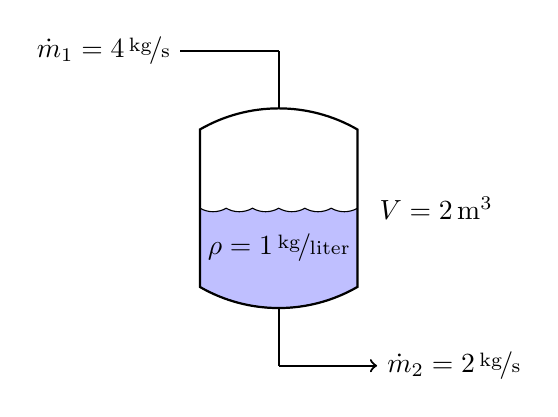
\begin{tikzpicture}
  %\draw[step=1cm,gray,very thin] (0,0) grid (6,6);
  
  % Coordinates
  \coordinate (drum) at (1.5,3);
  \coordinate (feed) at (0.5,3);

  % Drum outline. Given location of the feed port, draws a drum with
  % stubs for the liquid and vapor lines located at ++(1,2) and ++(1,-2)
  \draw[fill=blue!25] (drum) ++(0,-1) arc (240:300:2cm) -- ++(0,1)
    arc(-60:-120:0.333cm) arc(-60:-120:0.334cm) arc(-60:-120:0.333cm) 
    arc(-60:-120:0.333cm) arc(-60:-120:0.334cm) arc(-60:-120:0.333cm);
  \draw[thick] (drum) --++(0,-1) arc (240:300:2cm)
    -- ++(0,2) arc (60:120:2cm) -- ++(0,-1);
  \draw[thick] (drum) ++(1,1.268) -- ++(0,0.732); 
  \draw[thick] (drum) ++(1,-1.268) --++ (0,-0.732);
  
  % connecting the units
  %\draw[->,thick] (feed) node [left] {$\dot{m}_1 = \unitfrac[4]{kg}{s}$} -- (drum);
  \draw[thick] (drum) ++ (1,2) -- ++(-1.25,0) 
    node [left] {$\dot{m}_1 = \unitfrac[4]{kg}{s}$};
  \draw[->,thick] (drum) ++ (1,-2) -- ++(1.25,0) 
    node [right] {$\dot{m}_2 = \unitfrac[2]{kg}{s}$};
  
  % label units
  \draw (drum) ++ (3,0) node {\shortstack{$V=\unit[2]{m^3}$}};
  \draw (drum) ++ (1,-0.5) node {$\rho = \unitfrac[1]{kg}{liter}$};
  
\end{tikzpicture}
\end{sansmath}
\end{document}